\PassOptionsToPackage{svgnames}{xcolor}
\documentclass[8pt]{article}



\usepackage[margin=.1in]{geometry}  
\usepackage{graphicx}             
\usepackage{amsmath}              
\usepackage{amsfonts}              
\usepackage{framed}               
\usepackage{amssymb}
\usepackage{array}
\usepackage{amsthm}
\usepackage[nottoc]{tocbibind}
\usepackage{bm}
\usepackage[object=vectorian]{pgfornament} 
\usepackage{enumitem}

\colorlet{shadecolor}{lightgray!25}
\newcommand{\sectionline}{%
  \noindent
  \begin{center}
  {\color{DarkViolet}
    \resizebox{0.5\linewidth}{1ex}
    {{%
    {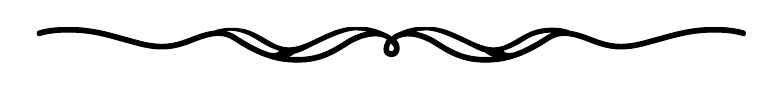
\begin{tikzpicture}
    \node  (C) at (0,0) {};
    \node (D) at (9,0) {};
    \path (C) to [ornament=85] (D);
    \end{tikzpicture}}}}}%
    \end{center}
  }

 \newcommand{\im}{\mathrm{i}}
  \newcommand{\diff}{\mathrm{d}}
\setlength{\parindent}{0cm}
\setlength{\parskip}{0em}
\newcommand{\Lim}[1]{\raisebox{0.5ex}{\scalebox{0.8}{$\displaystyle \lim_{#1}\;$}}}
\newtheorem{definition}{Definition}[section]
\newtheorem{theorem}{Theorem}[section]
\newtheorem{lemma}{Lemma}[section]
\newtheorem{corollary}{Corollary}[section]
\theoremstyle{definition}
\DeclareMathOperator{\arcsec}{arcsec}
\DeclareMathOperator{\arccot}{arccot}
\DeclareMathOperator{\arccsc}{arccsc}
\setcounter{tocdepth}{1}
\begin{document}

%\title{Revision notes - MA2108}
%\author{Ma Hongqiang}
%\maketitle
%\tableofcontents

%\clearpage

\section{The Real Number}
\subsection{Number Systems}
Examples of number systems include:
\begin{itemize}
\item $\mathbb{N}:=$ set of all \textbf{natural numbers} $={1,2,3,\cdots}$
\item $\mathbb{Z}:=$ set of all \textbf{integers} $= {\cdots,-3,-2,-1,0,1,2,3,\cdots}$
\item $\mathbb{Q}:=$ set of all \textbf{rational numbers} $= \{\frac{p}{q}\mid p,q\in\mathbb{Z},q\neq 0\}$
\item $\mathbb{R}:=$ set of all \textbf{real numbers}.
\end{itemize}
\begin{theorem}
\normalfont $\sqrt{2}$ is an irrational number.
\end{theorem}
\subsection{Natural Numbers}
$\mathbb{N}$ has the \textit{well-ordering property}:
\begin{center}
\fbox{\begin{minipage}{25em}
Every non-empty subset $S$ of $\mathbb{N}$ has a \textbf{minimum} element, i.e., there exists $m\in S$ such that $m\leq n$ for every $n\in S$.
\end{minipage}}
\end{center}
\begin{theorem}[Principle of Mathematical Induction]
\hfill\\\normalfont Let $S\subseteq\mathbb{N}$. If
\begin{enumerate}[label=(\roman*)]
\item $1\in S$, and
\item for every $k\in\mathbb{N}, k\in S\Rightarrow k+1\in S$,
\end{enumerate}
then $S=\mathbb{N}$.
\end{theorem}
\textbf{Remark}: The Theorem can be rephrasesd as:\\
For each $n\in\mathbb{N}$, let $P(n)$ be a statement about $n$. Suppose that
\begin{enumerate}[label=(\roman*)]
\item $P(1)$ is true, and 
\item for every $k\in\mathbb{N}$, if $P(k)$ is true, then $P(k+1)$ is true.
\end{enumerate}
Then $P(n)$ is true for every $n\in\mathbb{N}$.
\subsection{The Algebraic Properties of $\mathbb{R}$}
The binary operation \textbf{addition}(denoted by $+$) on the set $\mathbb{R}$ of real numbers satisfies the following properties:
\begin{enumerate}[label=(A\arabic*)]
\item \textbf{(Commutativity)} $a+b=b+a$ for all $a,b\in\mathbb{R}$.
\item \textbf{(Associativity)} $(a+b)+c=a+(b+c)$ for all $a,b,c\in\mathbb{R}$
\item \textbf{(Existence of zero element)} There exists a zero element $0\in\mathbb{R}$ such that $a+0=0+a=a$ for all $a\in\mathbb{R}$
\item \textbf{(Existence of inverse)} For each $a\in\mathbb{R}$, there exists an element $-a\in\mathbb{R}$ such that $a+(-a)=(-a)+a=0$.
\end{enumerate} 
Similarly, the binary operation \textbf{multiplication}(denoted by $\cdot$ or $\times$) on the set $\mathbb{R}$ satisfies the following properties:
\begin{enumerate}[label=(M\arabic*)]
\item \textbf{(Commutativity)} $a\cdot b=b\cdot a$ for all $a,b\in\mathbb{R}$.
\item \textbf{(Associativity)} $(a\cdot b)\cdot c=a\cdot(b\cdot c)$ for all $a,b,c\in\mathbb{R}$
\item \textbf{(Existence of unit element)} There exists a unit element $1\in\mathbb{R}$ such that $1\neq 0$ and $a\cdot 1=1\cdot a=a$ for all $a\in\mathbb{R}$
\item \textbf{(Existence of inverse)} For each $a\neq 0$ in $\mathbb{R}$, there exists an element $\frac{1}{a}\in\mathbb{R}$ such that $a\cdot\frac{1}{a}=\frac{1}{a}\cdot a=1$.
\end{enumerate} 
In addition, the two binary operations satisfy the following property:
\begin{enumerate}[label=(D)]
\item \textbf{(Distributivity of multiplication over addition)} $a\cdot(b+c)=a\cdot b + a\cdot c$ for all $a,b,c\in\mathbb{R}$.
\end{enumerate}
Because of properties (A1)---(A4),(M1)---(M4) and (D), we say that $(\mathbb{R},+,\cdot)$ forms a field.
\begin{theorem}[Some properties of $\mathbb{R}$]
\hfill\\
\normalfont Let $a,b,c\in\mathbb{R}$
\begin{enumerate}[label=(\roman*)]
\item (\textit{Uniqueness of additive inverse}) If $a+b=0$, then $b=-a$.
\item (\textit{Uniqueness of multiplicative inverse}) If $a\cdot b = 1$ and $b\neq 0$, then $b=\frac{1}{a}$.
\item If $a+b=b$, then $a = 0$.
\item If $b\neq 0$ and $a\cdot b = b$, then $a = 1$.
\item $a\cdot 0 = 0$ for all $a\in\mathbb{R}$.
\item If $a\cdot b = 0$, then $a = 0$ or $b = 0$.
\item (\textit{Cancellative property}) If $a\neq 0$ and $a\cdot b = a\cdot c$, then $b = c$.
\end{enumerate}
\end{theorem}
\begin{theorem}[Order Properties of $\mathbb{R}$]
\hfill\\
\normalfont There is a binary relation $>$ on $\mathbb{R}$ which has the following properties:\\Let $a,b,c,d\in\mathbb{R}$.
\begin{enumerate}[label=(O\arabic*)]
\item If $a>b$, then $a+c>b+c$.
\item If $a>0$ and $b>0$, then $a\cdot b>0$.
\item (\textbf{Trichotomy Property}) If $a,b\in\mathbb{R}$, then exactly one of the following holds:
\[
a>b,\;\;\;\;\; a=b,\;\;\;\;\;b>a
\]
\item (\textbf{Transitive Property}) If $a>b$ and $b>c$, then $a>c$.
\end{enumerate}
The other oder relations $<,\geq,\leq$ can be defined in terms of $>$.
\end{theorem}
Because of the order relation satisfies (O1)---(O4), we say that $(\mathbb{R},+,\cdot,>)$ forms an \textbf{ordered field}.
\begin{theorem}[Some more properties of $\mathbb{R}$]
\hfill\\
\normalfont Let $a,b,c\in\mathbb{R}$. Then the following statements hold:
\begin{enumerate}[label=(\roman*)]
\item $a>b\Leftrightarrow a-b>0$. \\In particular, $c<0 \Leftrightarrow -c>0$
\item Exactly one of the following holds:
\[
a>0,\;\;\;\;\;a=0,\;\;\;\;\;a<0
\]
\item If $a>b$ and $c>0$, then $c\cdot a>c\cdot b$. \\If $a>b$ and $c<0$, then $c\cdot a<c\cdot b$.
\item If $a\geq b$ and $b\geq a$, then $a=b$.
\end{enumerate}
\end{theorem}
\begin{theorem}
\hfill\\
\normalfont 
\begin{enumerate}[label=(\roman*)]
\item If $a\in\mathbb{R}$ and $a\neq 0$, then $a^2>0$
\item $1>0$
\item If $n\in\mathbb{N}$, then $n>0$
\item If $a>0$, then $\frac{1}{a}>0$
\end{enumerate}
\end{theorem}
\begin{theorem}
\normalfont If $a\in\mathbb{R}$ is such that $0\leq a<\epsilon$ for every positive number $\epsilon$, then $a=0$.
\end{theorem}
\subsection{Intervals}
An interval is a subset $I$ of $\mathbb{R}$ with the following property:
\begin{center}
\fbox{\begin{minipage}{12em}
\centering
If $x,y\in I$ and $x<y$, then\\$x<t<y\Rightarrow t\in I$
\end{minipage}}
\end{center}
\subsection{Solving Inequalities}
THe following two rules are often useful in solving inequalities:
\begin{enumerate}[label=Rule \arabic*]
\item If $a\cdot b>0$, then either
\begin{enumerate}[label=(\roman*)]
\item $a>0$ and $b>0$, or
\item $a<0$ and $b<0$
\end{enumerate}
\item If $a\cdot b<0$, then either
\begin{enumerate}[label=(\roman*)]
\item $a>0$ and $b<0$, or
\item $a<0$ and $b>0$
\end{enumerate}
\end{enumerate}
\begin{theorem}[Bernoulli's inequality]\normalfont If $x\geq -1$, then
\[
(1+x)^n\geq 1+nx\;\forall n\in\mathbb{N}
\]
\end{theorem}
\begin{definition}\normalfont Let $n\geq 2$ and let $a_1,a_2,\ldots,a_n$ be positive numbers.
\begin{itemize}
\item The \textit{arithmetic mean} of $a_1,a_2,\ldots,a_n$ is defined as $A = \frac{ a_1+a_2+\ldots+a_n }{n}$.
\item The \textit{geometric mean} of $a_1,a_2,\ldots,a_n$ is defined as $G = (a_1a_2\cdots a_n)^{\frac{1}{n}}$
\item The \textit{harmonic mean} of  $a_1,a_2,\ldots,a_n$ is defined as $H = \frac{n}{\frac{1}{a_1}+\frac{1}{a_2}+\cdots+\frac{1}{a_n}}$
\end{itemize}
\end{definition}
\begin{theorem}[AM-GM-HM inequality]\hfill\\
\normalfont Let $A,G,H$ be the arithmetic mean, the geometric mean and the harmonic mean of the positive numbers $a_1,a_2,\ldots,a_n$ respectively. Then
\[
H\leq G\leq A
\]
Moreover, the equalities hold if and only if $a_1 = a_2 = \cdots = a_n$.
\end{theorem}
\subsection{Absolute Value}
\begin{definition}\normalfont Let $a\in\mathbb{R}$. The \textbf{absolute value} of $a$ is defined by
\begin{equation*}
|a|=\begin{cases}
x &\text{if } a> 0\\
-x &\text{if } a<0\\
0 &\text{if }a=0
\end{cases}
\end{equation*}
\end{definition}
\begin{theorem}[Properties of absolute value]\hfill\\
\normalfont For all $a,b,c\in\mathbb{R}$, the following statements hold:
\begin{enumerate}[label=(\roman*)]
\item $|a|\geq 0$, $a\leq |a|$ and $-a\leq |a|$
\item $|a|=0\Leftrightarrow a=0$
\item $|-a|=|a|$
\item $|ab|=|a|\cdot|b|$
\item $|a|^2 = a^2$
\item If $c\geq 0$, then $|a|\leq c\Leftrightarrow -c\leq a\leq c$
\item $-|a|\leq a\leq|a|$
\end{enumerate}
\end{theorem}
\begin{theorem}[Triangle inequality]
\hfill\\
\normalfont For all $a,b\in\mathbb{R}$, we have
\[
|a+b|\leq |a|+|b|
\]
\end{theorem}
\begin{corollary}
\hfill\\
\normalfont For all $a,b\in\mathbb{R}$, we have
\begin{enumerate}[label=(\roman*)]
\item $\bigl\lvert\lvert a\rvert -\lvert b\rvert \bigr\rvert\leq|a-b|$
\item $\lvert a\rvert -\lvert b\rvert \leq|a|+|b|$
\end{enumerate}
\end{corollary}
\begin{corollary}\normalfont For $a_1,a_2,\ldots,a_n\in\mathbb{R}$, we have
\[
|a_1+a_2+\cdots+a_n|\leq|a_1|+|a_2|+\cdots+|a_n|
\]
\end{corollary}
\clearpage
\section{The Completeness of Real Numbers}
\subsection{Boundedness}
\begin{definition}\normalfont A non-empty set of real numbers $S\subset\mathbb{R}$ is said to be \textbf{bounded above} if there exists some $M\in\mathbb{R}$ such that
\[
x\leq M\;\forall x\in S
\]
Such an $M$ is called a \textbf{upper bound} of $S$.
\end{definition} 
\begin{definition}\normalfont A non-empty set of real numbers $S\subset\mathbb{R}$ is said to be \textbf{bounded below} if there exists some $m\in\mathbb{R}$ such that
\[
m\leq x\;\forall x\in S
\]
Such an $m$ is called a \textbf{lower bound} of $S$.
\end{definition}
\begin{definition}\normalfont A non-empty set of real numbers $S$ is said to be \textbf{bounded} if it is both bounded above and bounded below.
\end{definition}
\subsection{Maximum and Minimum of a set of real numbers}
\begin{definition}[Maximum]
\hfill\\\normalfont For a non-empty set $S\subset \mathbb{R}$, one defines the \textbf{maximum} of $S$ to be the (necessarily unique) number $M$ such that
\begin{enumerate}[label = max-\roman*]
\item $M\in S$, and 
\item $M\geq x$ for all $x\in S$
\end{enumerate}
\end{definition}
\begin{definition}[Minimum]
\hfill\\\normalfont Similarly, the \textbf{minimum} of $S$ to be the (necessarily unique) number $m$ such that
\begin{enumerate}[label = min-\roman*]
\item $M\in S$, and 
\item $m\geq x$ for all $x\in S$
\end{enumerate}
\end{definition}
\textbf{Remark:}
\begin{enumerate}
\item If a set $S\subset\mathbb{R}$ has a maximum, then $S$ is bounded above, since by (max-ii), $\max S$ is an upper bound of $S$.\\Similarly if a set $S\subset\mathbb{R}$ has a minimum, then $S$ is bounded below.
\item If a set $S$ has a maximum, then $\max S$ is unique.
\end{enumerate}
\subsection{Infimum and Supremum}
\begin{definition}\normalfont Let $E$ be a non-empty set of real numbers. A real number $M\in\mathbb{R}$ is called the least upper bound or \textbf{supremum} of $E$ if
\begin{enumerate}[label=(S-\roman*)]
\item $M$ is an upper bound of $E$, i.e., $x\leq M\;\forall x\in E$, and
\item if $M^\prime$ is an upper bound of $E$, then $M^\prime\geq M$.
\end{enumerate}
\end{definition}
\begin{lemma}\normalfont Let $E$ be a non-empty set of real numbers. Then $M=\sup E$ if and only if $M$ satisfies (S-i) and
\begin{itemize}
\item[(S-ii'] for every $\epsilon>0$, there exists $x_\epsilon\in E$ such that $x_\epsilon>M-\epsilon$
\end{itemize}
\end{lemma}
\textbf{Remark:}
\begin{enumerate}[label=(\roman*)]
\item $\sup E$ is unique whenever it exists.
\item The main difference between $\sup E$ and $\max E$ is that $\sup E$ may not be an element of $E$, whereas $\max E$ must be an element of $E$, if it does exist.
\item If $E$ has a maximum, then $\sup E = \max E$.
\end{enumerate}
\begin{definition}\normalfont Let $E$ be a non-empty set of real numbers. A real number $m\in\mathbb{R}$ is called the greatest lower bound or \textbf{infimum} of the set $E$ if
\begin{enumerate}[label=(I-\roman*)]
\item $m$ is a lower bound of $E$, i.e., $m\leq x\;\forall x\in E$, and
\item if $m^\prime$ is a lower bound of $E$, then $m^\prime\leq m$.
\end{enumerate}
\end{definition}
\begin{lemma}\normalfont Let $E$ be a non-empty set of real numbers. Then $m=\inf E$ if and only if $m$ satisfies (I-i) and 
\begin{itemize}
\item[(I-ii')] for every $\epsilon>0$, there exists $x_\epsilon\in E$ such that $x_\epsilon<m+\epsilon$.
\end{itemize}
\end{lemma}
\textbf{Remark:}
\begin{enumerate}[label=(\roman*)]
\item $\inf E$ is unique whenever it exists.
\item The main difference between $\inf E$ and $\min E$ is that $\inf E$ may not be an element of $E$, whereas $\min E$ must be an element of $E$, if it does exist.
\item If $E$ has a minimum, then $\inf E = \min E$.
\end{enumerate}
\subsection{Completeness Property of $\mathbb{R}$}
\begin{theorem}\normalfont Every non-empty subset of $\mathbb{R}$ which is bounded above has a supremum in $\mathbb{R}$.
\end{theorem}
\subsubsection{Infimum property of $\mathbb{R}$}
\begin{theorem}\normalfont Every non-empty subset of $\mathbb{R}$ which is bounded below has an infimum in $\mathbb{R}$.
\end{theorem}
\subsubsection{Some consequences of the completeness of $\mathbb{R}$}
\begin{theorem}[Archimedian property of $\mathbb{R}$]\hfill\\\normalfont
For any $x\in\mathbb{R}$, there exists $n_x\in\mathbb{N}$ such that $x<n_x$.
\end{theorem}
\textbf{Remark:} The Archimedean property of $\mathbb{R}$ is equivalent to the statement that $\mathbb{N}$ is not bounded above in $\mathbb{R}$.
\begin{corollary}\hfill
\normalfont\begin{enumerate}
\item Let $A=\{\frac{1}{n}\mid n\in\mathbb{N}\}$. Then $\inf A=0$.
\item In particular, if $\epsilon>0$, then there exists $n_\epsilon\in\mathbb{N}$ such that $0<\frac{1}{n_\epsilon}<\epsilon$
\end{enumerate}
\end{corollary}
\begin{theorem}\normalfont Let $c>0$ and $k\in\mathbb{N}$. Then there exists a unique positive real number $a$ with $a^k=c$.
\end{theorem}
\begin{theorem}[The Density Theorem]
\hfill\\
\normalfont For any two \textbf{real} number $x,y\in\mathbb{R}$ satisfying $x<y$, there exists a \textbf{rational} number $r\in\mathbb{Q}$ such that
\[
x<r<y
\]
\end{theorem}
\begin{corollary}\normalfont If $a,b\in\mathbb{R}$ is such that $a<b$, then there exists $x\in\mathbb{R}\setminus\mathbb{Q}$ such that $a<x<b$.
\end{corollary}
\begin{corollary}\normalfont If an interval $I\subseteq \mathbb{R}$ has at least two elements, then $I$ contains infinitely many rational numbers and infinitely many irrational numbers. 
\end{corollary}
\begin{definition}\normalfont A subset $D$ of $\mathbb{R}$ is said to be \textbf{dense} in $\mathbb{R}$ if for any $a,b\in\mathbb{R}$ with $a<b$, $D\cap(a,b)\neq\varnothing$
\end{definition}
\textbf{Remark}: Both $\mathbb{Q}$ and $\mathbb{R}\setminus\mathbb{Q}$ are dense in $\mathbb{R}$.
\subsection{More on Intervals}
\begin{theorem}\normalfont Every interval belongs to one of the following 9 types:
\[
\begin{aligned}
(a,b)&=\{x\in\mathbb{R}:a<x<b\}\\
[a,b]&=\{x\in\mathbb{R}:a\leq x\leq b\}\\
[a,b)&=\{x\in\mathbb{R}:a\leq x<b\}\\
(a,b]&=\{x\in\mathbb{R}:a<x\leq b\}\\
[a,\infty)&=\{x\in\mathbb{R}:x\geq a\}\\
(a,\infty)&=\{x\in\mathbb{R}:x>a\}\\
(-\infty,b]&=\{x\in\mathbb{R}:x\leq b\}\\
(-\infty,b)&=\{x\in\mathbb{R}:x<b\}\\
(-\infty,\infty)=\mathbb{R}
\end{aligned}
\]
\end{theorem}
\begin{definition}\normalfont A sequence of intervals $I_n, n\in\mathbb{N}$, is said to be \textbf{nested} if $I_n\supseteq I_{n+1}$ for each $n\in\mathbb{N}$.
\[
I_i\supseteq I_2\supseteq \cdots \supseteq I_n\supseteq I_{n+1}\supseteq \cdots
\]
\end{definition}
\begin{theorem}[Nested Interval Property]
\hfill\\\normalfont If $I_n=[a_n,b_n], n\in\mathbb{N}$, is a nested sequence of non-empty closed bounded intervals, then there exists a number $\xi\in\mathbb{R}$ such that $\xi\in I_n$ for all $n\in\mathbb{N}$,i.e. $\cap_{n=1}^\infty I_n\neq\varnothing$.
\end{theorem}
\begin{theorem}\normalfont If $I_n=[a_n,b_n],n\in\mathbb{N}$, is a nested sequence of non-empty closed bounded intervals, and the length $b_n-a_n$ of $I_n$ satisfy
\[
\inf\{b_n-a_n:n\in\mathbb{N}\}=0
\]
then $\cap_{n=1}^\infty I_n$ has exactly one element.
\end{theorem}
\begin{theorem}\normalfont Let $I=[0,1]$. There does not ecists a bijection $f:\mathbb{N}\to I$ from $\mathbb{N}$ onto $I$.
\end{theorem}
\clearpage
\section{Sequences}
\begin{definition}
\hfill\\\normalfont A \textbf{sequence} in $\mathbb{R}$ is a real-valued function $X$ with demain $\mathbb{N}$, that is
\[
X:\mathbb{N}\to\mathbb{R}
\]
The numbers $X(n)$ for $n=1,2,3,\ldots$ are called the terms of the sequence $X$ by $(x_n)$.
\end{definition}
\begin{definition}[Limit of sequence]
\hfill\\\normalfont We say that $x$ is the \textbf{limit} of $(x_n)$ if for every $\epsilon>0$, there exists $K=K(\epsilon)\in\mathbb{N}$ such that
\[
|x_n-x|<\epsilon\forall n\geq K
\]
\end{definition}
\begin{definition}[Convergence and Divergence]
\hfill\\\normalfont If $x$ is the limit of $(x_n)$, then we aso say that $(x_n)$ \textbf{converges} to $x$, and we write
\[
\Lim{n\to\infty}x_n=x
\] 
We say that a sequence $(x_n)$ \textbf{converges}, if $(x_n)$ converges to a \textbf{finite} limit $x\in\mathbb{R}$.\\
We say that a sequence $(x_n)$ \textbf{diverges} if $(x_n)$ does not converge.
\end{definition}
\begin{theorem}\normalfont If $(x_n)$ converges, then it has exactly one limit.
\end{theorem}
\subsection{Limit Theorems}
\begin{definition}\normalfont A sequence $(x_n)$ is said to be \textbf{bounded} if there exists $M>0$ such that
\[
|x_n|\leq M\;\;\;\forall n\in\mathbb{N}
\]
\end{definition}
\begin{theorem}\normalfont Every convergent sequence is bounded.\end{theorem}
\begin{theorem}
\hfill\\\normalfont If $\Lim{n\to\infty}x_n=x$ and $\Lim{n\to\infty}y_n = y$, then
\begin{enumerate}
\item $\Lim{n\to\infty}(x_n+y_n)=x+y$
\item $\Lim{n\to\infty} x_n y_n = xy$
\item $\Lim{n\to\infty}\frac{x_n}{y_n}=\frac{x}{y}$, provided $y_n\neq 0\;\forall n\in\mathbb{N}$, and $y\neq 0$.
\end{enumerate}
\end{theorem}
\begin{corollary}\normalfont If $(x_n)$ converges and $k\in\mathbb{N}$, then
\[
\Lim{n\to\infty}x^k_n=\left(\Lim{n\to\infty}x_n\right)^k
\]
\end{corollary}
\begin{theorem}[Squeeze Theorem]
\hfill\\\normalfont If $x_n\leq y_n\leq z_n$ for all $n\in \mathbb{N}$ and $\Lim{n\to \infty}x_n=\Lim{n\to\infty}z_n = a$. Then,
\[
Lim{n\to\infty} y_n =a
\]
\end{theorem}
Remark: the conditon "$x_n\leq y_n\leq z_n$ for all $n\in \mathbb{N}$" can be replaced by weaker condition $x_n\leq y_n \leq z_n$ for all natural numbers $n\geq K_0$.
\begin{theorem}
\normalfont If $|x_n|\to 0$, then $x_n\to 0$.
\end{theorem}
\begin{theorem}
\normalfont If $0<b<1$, then $\Lim{n\to\infty} b^n=0$.
\end{theorem}
\begin{theorem}
\normalfont If $c>0$, then $\Lim{n\to\infty}c^\frac{1}{n}=1$
\end{theorem}
\begin{theorem}
\normalfont
\begin{enumerate}
\item If $\Lim{n\to\infty}x_n= x$, then $\Lim{n\to\infty}|x_n|= |x|$.
\item If all $x_n\geq 0$ and $\Lim{n\to\infty}x_n = x$, then $\Lim{n\to\infty}\sqrt{x_n}=\sqrt{x}$.
\end{enumerate}
\end{theorem}
\begin{theorem}
\[
\Lim{n\to\infty}n^\frac{1}{n}=1
\]
\end{theorem}
\begin{theorem}
\normalfont
\begin{enumerate}
\item If $x_n\geq 0$ for all $n\in\mathbb{N}$, and $(x_n)$ converges, then $\Lim{n\to\infty}x_n\geq 0$.
\item If $(x_n)$ and $(y_n)$ are convergent and $x_n\geq y_n$ for all $n\in\mathbb{N}$, then
\[
\Lim{n\to\infty} x_n\geq \Lim{n\to\infty}y_n
\]
\item If $a,b\in\mathbb{R}$, and $a\leq x_n\leq b$ for all $n$ and $(x_n)$ is convergent, then
\[
a\leq \Lim{n\to\infty}x_n\leq b
\]
\end{enumerate}
\end{theorem}
\subsection{Monotone Sequences}
\begin{definition}\normalfont We say that the sequence $(x_n)$ is
\begin{itemize}
\item \textbf{increasing} if
\[
x_1\leq x_2\leq\cdots\leq x_n\leq x_{n+1}\leq \cdots
\]
\item \textbf{decreasing} if
\[
x_1\geq g_2\geq\cdots\geq x_n\geq x_{n+1}\geq \cdots
\]
\item \textbf{monotone} if it is either increasing and decreasing
\end{itemize}
\end{definition}
\begin{theorem}[Monotone Convergence Theorem]
\hfill\\\normalfont If $(x_n)$ is monotone and bounded, then it is convergent. In this case,
\[
\Lim{n\to\infty}x_n = 
\begin{cases}
\sup\{x_n\mid n\in\mathbb{N}\}\text{ if }x_n\text{ is increasing}\\
\inf\{x_n\mid n\in\mathbb{N}\}\text{ if }x_n\text{ is decreasing}
\end{cases}
\]
\end{theorem}
\begin{corollary}
\begin{enumerate}
\item If $(x_n)$ is increasing and bounded above, then it converges and 
\[
\Lim{n\to\infty}x_n = \sup\{x_n\mid n\in\mathbb{N}\}
\]
\item If $(x_n)$ is decreasing and bounded below, then it converges and 
\[
\Lim{n\to\infty}x_n = \inf\{x_n\mid n\in\mathbb{N}\}
\]
\end{enumerate}
\end{corollary}
\subsection{Subsequences and the Bolzano-Weierstrass Theorem}
\begin{definition}[Subsequence]
\hfill\\\normalfont Let $(x_n)$ be a sequence and let
\[
n_1\leq n_2\leq \cdots\leq n_k\leq n_{k+1}\leq \cdots
\]
be an increasing sequence of natural numbers. The sequence
\[
(x_{n_k})=(x_{n_1},x_{n_2},\cdots,x_{n_k},\cdots)
\]
is called a subsequence of $(x_n)$.
\end{definition}
\begin{theorem}\normalfont If $(x_n)$ converges to $x$, then any subsequence $(x_{n_k})$ also converges to $x$.
\end{theorem}
\begin{corollary}\normalfont If $(x_n)$ has a subsequence which is divergent, then $(x_n)$ diverges.
\end{corollary}
\begin{corollary}\normalfont If $(x_n)$ has two convergent subsequences whose limits are not equal, then $(x_n)$ diverges.
\end{corollary}
\begin{theorem}[Monotone Subsequence Theorem]
\hfill\\\normalfont Every sequence has a monotone subsequence.
\end{theorem}
\begin{theorem}[Bolzano-Weierstrass Theorem]
\hfill\\\normalfont Every bounded sequence has a convergent subsequence.
\end{theorem}
\subsection{Limit superior and limit inferior}
\begin{definition}\normalfont Let $(x_n)$ be a sequence of real numbers. A real number $x$ is called a \textbf{subsequential limit} of $(x_n)$ if $(x_n)$ has a subsequence $(x_{n_k})$ which converges to $x$, that is,
\[
x_{n_k}\to x
\]
\end{definition}
\begin{definition}\normalfont Let $S(x_n)$ denote the set of all subsequential limits of $(x_n)$.
\end{definition}
\begin{definition}\normalfont
\begin{enumerate}
\item We define the \textbf{limit superior} of $(x_n)$ to be
\[
\lim\sup x_n:=\sup S(x_n)
\]
\item We define the \textbf{limit inferior} of $(x_n)$ to be
\[
\lim\inf x_n:=\inf S(x_n)
\]
\end{enumerate}
\end{definition}
\begin{theorem}\normalfont Let $(x_n)$ be a bounded sequence and let $M = \lim\sup x_n$.
\begin{enumerate}
\item For each $\epsilon>0$, there are at most finitely many $n$'s such that $x_n\geq M+\epsilon$.\\
Equivalently, for each $\epsilon>0$, there exists $K\in\mathbb{N}$ such that
\[
x_n<M+\epsilon\;\;\;\;\forall n\geq K
\]
\item For each $\epsilon>0$, there are infinitely many $n$'s such that $x_n> M-\epsilon$.
\end{enumerate}
The converse is also true.
\end{theorem}
\begin{theorem}\normalfont Let $(x_n)$ be a bounded sequence and let $m = \lim\inf x_n$.
\begin{enumerate}
\item For each $\epsilon>0$, there are at most finitely many $n$'s such that $x_n\leq m-\epsilon$.\\
Equivalently, for each $\epsilon>0$, there exists $K\in\mathbb{N}$ such that
\[
x_n>m-\epsilon\;\;\;\;\forall n\geq K
\]
\item For each $\epsilon>0$, there are infinitely many $n$'s such that $x_n< m+\epsilon$.
\end{enumerate}
The converse is also true.
\end{theorem}
\begin{theorem}[Equivalent definition of $\lim\sup$]
\hfill\\\normalfont 
If $(x_n)$ is a bounded sequence of real numbers, then the following statements for a real number $x^\ast$ are equivalent.
\begin{enumerate}
\item $x^\ast = \lim\sup (x_n)$. The limit superior of $(x_n)$ is the infimum of the set $V$ of $v\in\mathbb{R}$ such that $v<x_n$ for at most a finite number of $n\in\mathbb{N}$.
\item If $\epsilon>0$, there are at most a finite number of $n\in\mathbb{N}$ such that $x^\ast+\epsilon<x_n$, but an infinite number of $n\in\mathbb{N}$ such that $x^\ast-\epsilon<x_n$.
\item If $u_m=\sup\{x_n\mid n\geq m\}$, then $x^\ast = \inf \{u_m\mid m\in\mathbb{N}\} = \lim(u_m)$.
\item If $S$ is the set of subsequential limits of $(x_n)$, then $x^\ast = \sup S$.
\end{enumerate}
\end{theorem}
\begin{theorem} \normalfont Let $(x_n)$ be a bounded sequence. Then $(x_n)$ converges if and only if
\[
\lim\sup x_n=\lim\inf x_n
\]
\end{theorem}
\begin{theorem}\normalfont Let $(x_n)$ and $(y_n)$ be bounded sequences such that $x_n\leq y_n$ for every $n\in\mathbb{N}$. Then,
\[
\lim\sup x_n\leq \lim\sup y_n
\]
and
\[
\lim\inf x_n\leq \lim\inf y_n
\]
\end{theorem}
\subsection{The Cauchy Criterion}
\begin{definition}\normalfont A sequence $(x_n)$ is called a \textbf{Cauchy sequennce} if for every $\epsilon>0$, there exists $K=K(\epsilon)\in\mathbb{N}$ such that
\[
|x_n-x_m|\leq \epsilon \;\;\;\forall n,m\geq K
\]
\end{definition}
\begin{theorem}\normalfont Every convergent sequence is Cauchy.
\end{theorem}
\begin{theorem}\normalfont Every Cauchy sequence is bounded.
\end{theorem}
\begin{theorem}[Cauchy Criterion]
\hfill\\\normalfont Every Cauchy sequence is convergent.
\end{theorem}
\begin{definition}\normalfont A sequence $(x_n)$ is said to be \textbf{contractive} if there exists $C$ with $0<C<1$ such that
\[
|x_{n+2}-x_{n+1}|\leq C|x_{n+1}-x_n|\;\;\;\forall n\in\mathbb{N}
\]
\end{definition}
\begin{theorem}\normalfont Every contractive sequence is Cauchy.
\end{theorem}
\subsection{Properly Divergent Sequences}
\begin{definition}\normalfont We say that a sequence $(x_n)$ \textbf{tends to} $\infty$ if for every $M>0$, there exists $K=K(M)\in\mathbb{N}$ such that
\[
x_n>M\;\;\;\forall n\geq K
\]
In this case,we write
\[
\Lim{n\to\infty} x_n = \infty
\]
\end{definition}
\textbf{Remark}: If a sequence $(x_n$) is increasing and unbounded, then $x_n\to\infty$.
\begin{definition}\normalfont We say that a sequence $(x_n)$ \textbf{tends to} $-\infty$ if for every $M<0$, there exists $K=K(M)\in\mathbb{N}$ such that
\[
x_n<M\;\;\;\forall n\geq K
\]
In this case,we write
\[
\Lim{n\to\infty} x_n = -\infty
\]
\end{definition}
\begin{definition}\normalfont We call a sequence $(x_n)$ \textbf{properly divergent} if either $x_n\to\infty$ or $x_n\to -\infty$.
\end{definition}
\begin{definition}[$o(x_n)$]
\hfill\\\normalfont Let $(x_n)$ and $(y_n)$ be two sequences of positive numbers such that $\Lim{n\to\infty}x_n=\infty$ and $\Lim{n\to\infty} y_n=\infty$. We write,
\[
x_n=o(y_n) \text{ and also }x_n\ll y_n\text{ if }\Lim{n\to\infty}\frac{x_n}{y_n}=0 
\] 
\end{definition}
\textbf{Remark}: $n^k\ll a^n\ll n!$
\clearpage
\section{Infinite Series}
\begin{definition}\normalfont Given a series $\sum_{k=1}^\infty a_k$, its $n$th \textbf{partial sum} $s_n$ is given by
\[
s_n=\sum_{k=1}^n a_k = a_1+a_2+\cdots+a_n
\]
The sequence $(s_n)$ is called \textbf{the sequence of partial sums} of the series $\sum_{k=1}^\infty a_k$.
\end{definition}
\begin{definition}\normalfont Consider the sequence of partial sums $(s_n)$ of the series $\sum_{k=1}^\infty a_k$. If the sequence $(s_n)$ converges to a number $S\in\mathbb{R}$, we say that the series $\sum_{k=1}^\infty a_k$ \textbf{converges} to $S$ and write
\[
\sum_{k=1}^\infty a_k = \Lim{n\to\infty}s_n=S
\]
In this case, $S$ is called the \textbf{sum} of the seriess $\sum_{k=1}^\infty a_k$.\\
If $(s_n)$ diverges, then we say $\sum_{k=1}^\infty a_k$ \textbf{diverges}.
\end{definition}
\begin{definition}[Geometric Series]
\hfill\\\normalfont Let $a\neq 0$ and $r$ be fixed real numbers. Consider the geometric series
\[
\sum_{k=1}^\infty ar^{k-1} = a+ar+ar^2+\cdots
\]
Here $r$ is called the \textbf{common ratio} of the series.\\
In summary, the \textbf{geometric series}
\[
\sum_{k=1}^\infty ar^{k-1}=\begin{cases}
\frac{a}{1-r},&\text{ if }|r|<1\\
\textbf{diverges}&\text{ if }|r|\geq 1
\end{cases}
\]
\end{definition}
\begin{theorem}[Linear Combination of convergent sequences is convergent]
\hfill\\\normalfont
\begin{enumerate}
\item If the series $\sum_{n=1}^\infty a_n$ and $\sum_{n=1}^\infty b_n$ are convergent, then the series $\sum_{n=1}^\infty (a_n+b_n)$ is also convergent and  $\sum_{n=1}^\infty (a_n+b_n)=\sum_{n=1}^\infty a_n+\sum_{n=1}^\infty b_n$.
\item If the series $\sum_{n=1}^\infty a_n$ is convergent and $c\in\mathbb{R}$, then the series $\sum_{n=1}^\infty ca_n$ is also convergent and $\sum_{n=1}^\infty ca_n=c\sum_{n=1}^\infty a_n$.
\end{enumerate}
\end{theorem}
\begin{theorem}\normalfont If $\sum_{n=1}^\infty a_n$ converges, then $\Lim{n\to\infty} a_n=0$.
\end{theorem}
\begin{theorem}[The $n$th term divergence test]
\hfill\\\normalfont
\begin{enumerate}
\item If $\Lim{n\to\infty} a_n\neq 0$, then $\sum_{n=1}^\infty a_n$ diverges.
\item If $\Lim{n\to\infty} a_n= 0$, then NO conclusion for $\sum_{n=1}^\infty a_n$ can be drawn.
\end{enumerate}
\end{theorem}
\begin{theorem}[Cauchy Criterion for Series]
\hfill\\\normalfont
The series $\sum_{n=1}^\infty a_n$ converges if and only if for every $\epsilon>0$, there exists $K=K(\epsilon)\in\mathbb{N}$ such that
\[
|a_{n+1}+a_{n+2}+\cdots+a_m|<\epsilon\;\;\;\text{for all }m>n\geq K
\]
\end{theorem}
\subsection{Series with nonnegative terms}
\begin{definition}\normalfont A series $\sum_{k=1}^\infty a_k$ is called an \textbf{eventually nonnegative series} if each term $a_k\geq 0$. Here $a_k\geq 0$ eventually means there exists $K\in\mathbb{N}$ such that $a_k\geq 0$ for all $k\geq K$.
\end{definition}
\begin{theorem}\normalfont Let $\sum_{n=1}^\infty a_n$ be an (eventually) non-negative series. Then $\sum_{n=1}^\infty a_n$ converges if and only if the sequences $(s_n)$ of partial sums if bounded.
\end{theorem}
\begin{theorem}\normalfont If $p>1$, then $p$-series $\sum_{n=1}^\infty \frac{1}{n^p}$ converges.
\end{theorem}
\begin{theorem}[Comparison Test]
\hfill\\\normalfont Consider 2 nonnegative series $\sum_{k=1}^\infty a_k$ and $\sum_{k=1}^\infty b_k$. Suppose that there exists $K\in\mathbb{N}$ such that
\[
0\leq a_k\leq b_k\;\;\;\text{for all }k\geq K
\] 
\begin{enumerate}
\item If $\sum_{k=1}^\infty b_k$ converges, then $\sum_{k=1}^\infty a_k$ converges.
\item If $\sum_{k=1}^\infty a_k$ diverges, then $\sum_{k=1}^\infty b_k$ diverges.
\end{enumerate}
\end{theorem}
\begin{theorem}\normalfont If $p\leq 1$, then the $p$-series $\sum_{n=1}^\infty \frac{1}{n^p}$ diverges.
\end{theorem}
\begin{theorem}[Limit Comparison Test]
\hfill\\\normalfont Let $\sum_{n=1}^\infty a_n$ and $\sum_{n=1}^\infty b_n$ be two eventually positive series, and suppose that the limit
\[
\rho = \Lim{n\to\infty}\frac{a_n}{b_n}
\]
exists.
\begin{enumerate}
\item If $\rho>0$, then either the two series both converge or both diverge.
\item If $\rho=0$ and $\sum_{n=1}^\infty b_n$ converges, then $\sum_{n=1}^\infty a_n$ converges.
\end{enumerate}
\end{theorem}
\begin{theorem}[Ratio Test]
\hfill\\\normalfont Let $\sum_{n=1}^\infty a_n$ be eventually positive series and suppose that the limit
\[
\rho = \Lim{n\to\infty}\frac{a_{n+1}}{a_n}
\]
exists.
\begin{enumerate}
\item If $\rho<1$, then the series $\sum_{n=1}^\infty a_n$ converges.
\item Ig $\rho>1$, then the series $\sum_{n=1}^\infty a_n$ diverges.
\item No conclusion if $\rho = 1$.
\end{enumerate}
\end{theorem}
\begin{theorem}[Root Test]
\hfill\\\normalfont Let $\sum_{n=1}^\infty a_n$ be an eventually non-negative series, and suppose $(a_n^{\frac{1}{n}})$ is a bounded sequence. Let
\[
\rho = \lim\sup a_n^{\frac{1}{n}}
\]
\begin{enumerate}
\item If $\rho<1$, then the series $\sum_{n=1}^\infty a_n$ converges.
\item Ig $\rho>1$, then the series $\sum_{n=1}^\infty a_n$ diverges.
\item No conclusion if $\rho = 1$.
\end{enumerate}
\end{theorem}
\begin{theorem}[Simplified Root Test]
\hfill\\\normalfont Let $\sum_{n=1}^\infty a_n$ be an eventually non-negative series. Suppose
\[
\rho = \Lim{n\to\infty} a_n^{\frac{1}{n}}
\]
\begin{enumerate}
\item If $\rho<1$, then the series $\sum_{n=1}^\infty a_n$ converges.
\item If $\rho>1$, then the series $\sum_{n=1}^\infty a_n$ diverges.
\item No conclusion if $\rho = 1$.
\end{enumerate}
\end{theorem}
\subsection{Alternating series}
\begin{definition}\normalfont An \textbf{alternating series} is a series of the form
\[
\begin{aligned}
\sum_{k=1}^\infty (-1)^k a_k&=a_1-a_2+a_3-a_4+\cdots,\;\;\;\text{or}\\
\sum_{k=1}^\infty (-1)^{k+1} a_k&=-a_1+a_2-a_3+a_4-\cdots
\end{aligned}
\]
with each $a_k\geq 0$.
\end{definition}
\begin{theorem}[Alternating series Test]
\hfill\\\normalfont Let $\sum_{n=1}^\infty (-1)^{n+1}a_n$ or $\sum_{n=1}^\infty (-1)^{n}a_n$ be an alternating series. Suppose that
\begin{enumerate}
\item $a_n\geq 0$ for all $n$,
\item $(a_n)$ is decreasing, and
\item $\Lim{n\to infty}a_n = 0$.
\end{enumerate}
Then $\sum_{n=1}^\infty (-1)^{n+1}a_n$ or $\sum_{n=1}^\infty (-1)^{n}a_n$ is convergent.
\end{theorem}
\subsection{Series with both positive and negative terms}
\begin{definition}\hfill\\\normalfont
\begin{enumerate}
\item We say that the series $\sum_{n=1}^\infty a_n$ \textbf{converges absolutely} if the series $\sum_{n=1}^\infty |a_n|$ converges.
\item We say that the series $\sum_{n=1}^\infty a_n$ \textbf{converges conditionally} if 
\begin{enumerate}
\item $\sum_{n=1}^\infty a_n$ converges, and
\item $\sum_{n=1}^\infty |a_n|$ diverges.
\end{enumerate}
\end{enumerate}
\end{definition}
\begin{theorem}\normalfont If the series $\sum_{n=1}^\infty a_n$ converges absolutely, then it converges.
\end{theorem}
\begin{theorem}\normalfont Every series is either absolutely convergent, conditionally convergent or divergent.
\end{theorem}
\subsection{Grouping of series}
\begin{theorem}\normalfont If the series $\sum_{n=1}^\infty a_n$ converges, then any series obtained by grouping the terms of $\sum_{n=1}^\infty a_n$ is also convergent and has the same sum as $\sum_{a=1}^\infty a_n$.
\end{theorem}
\subsection{Rearrangement of series}
\begin{definition}\normalfont A series $\sum_{n=1}^\infty b_n$ is a \textbf{rearrangement} of the series $\sum_{n=1}^\infty a_n$ if there is a bijection $f:\mathbb{N}\to\mathbb{N}$ such that $b_n=a_{f(n)}$ for all $n\in \mathbb{N}$.
\end{definition}
\begin{theorem}\normalfont If the series $\sum_{n=1}^\infty a_k$ converges absolutely, then any rearrangement $\sum_{n=1}^\infty b_k$ of $\sum_{n=1}^\infty a_k$ also converges and has the same sum as $\sum_{n=1}^\infty a_n$.
\end{theorem}
 
\section{Limits of Functions}
\subsection{Definition of Limits}
\begin{definition}\normalfont Let $\varnothing\neq A\subset\mathbb{R}$. A number $c\in\mathbb{R}$ is said to be a \textbf{cluster point} of $A$ if for every $\delta>0$, the open interval $(c-\delta, c+\delta)$ contains a point of $A\setminus\{c\}$.
\end{definition}
\begin{theorem}\normalfont A real number $c$ is a cluster point of $\varnothing\neq A\subset \mathbb{R}$ if and only if there exists a sequence $(a_n)$ in $A\setminus\{c\}$ converging to $c$.
\end{theorem}
\begin{definition}[$\epsilon$--$\delta$ definition of limit]
\hfill\\\normalfont Let $f:A\to \mathbb{R}$ be a function, where $\varnothing\neq A\subset \mathbb{R}$, and let $c$ be a cluster point of $A$. We say that a real number $L$ is the \textbf{limit} of $f$ at $x=c$ and write
\[
\Lim{x\to c}f(x)=L
\]
if for every $\epsilon>0$, there exists $\delta = \delta(\epsilon)>0$ such that
\[
|f(x)-L|<\epsilon\;\;\;\text{for all }x\in A\text{ satisfying }0<|x-c|<\delta 
\]
In this case, we also say that $f$ \textbf{converges} to $L$ at $x=a$.
\end{definition}
\begin{definition}\normalfont If $h>0$, then the $h$-\textbf{neighbourhood} of the point $a$ is the set
\[
V_h(a)=\{x:|x-a|<h\}=(a-h,a+h)
\]
Define
\[
V_h^\ast(a)=V_h(a)\setminus \{a\}=\{x:0<|x-a|<h\}
\]
$V_h^\ast(a)$ is called a \textbf{deleted neighbourhood} of $a$.
\end{definition}
\textbf{Remark:} Let $f:A\to\mathbb{R}$ be a function, and let $c$ be a cluster point of $A$ as before. Then the definition of limit can be restated as follows: $\Lim{x\to c}f(x)=L$ if and only if for any given $\epsilon>0$, there exists $\delta=\delta(\epsilon)>0$ such that
\[
f(A\cap V_\delta^\ast(c))\subset V_\epsilon(L)
\]
\begin{theorem}[Sequential Criterion for Limits]
\hfill\\\normalfont Let $\varnothing\subsetneq A\subset\mathbb{R}$, and let $c$ be a cluster point of $A$. Suppose that $f:A\to \mathbb{R}$ is a function and $L\in\mathbb{R}$. Then the following statements are equivalent.
\begin{enumerate}
\item $\Lim{x\to c}f(x)=L$
\item For every seqeuence $(x_n)$ in $A\setminus\{c\}$ satisfying $\Lim{n\to\infty}x_n = c$, one has $\Lim{n\to\infty}f(x_n)=L$.
\end{enumerate}
\end{theorem}
\begin{theorem}[Uniqueness of Limits]
\hfill\\\normalfont If $f:A\to\mathbb{R}$ is a function and $c$ is a cluster point of $A$, then the limit of $f$ at $x=c$ is unique, if it does exist. In other words, if $\Lim{x\to c}f(x)=L_1$ and $\Lim{x\to c}f(x)=L_2$ also, then $L_1 = L_2$.
\end{theorem}
\begin{theorem}\normalfont Let $f:A\to\mathbb{R}$ be a function, and let $c$ be a cluster point of $A$. Then $\Lim{x\to c}f(x)\neq L\Leftrightarrow$ there is a sequence $(x_n)$ in $A\setminus\{c\}$ such that $x_n\to c$, but $f(x_n)$ does not converge to $L$.
\end{theorem}
\begin{theorem}[Divergence Criteria]
\hfill\\\normalfont Let $f:A\to\mathbb{R}$ be a function, and let $c$ be a cluster point of $A$. To prove that $\Lim{x\to c}f(x)$ does not exist:
\begin{enumerate}[label = Method \arabic*]
\item Find a sequence $(x_n)$ in $A\setminus\{c\}$ such that $x_n\to c$, but the sequence $(f(x_n))$ diverges.
\item Find two sequences $(x_n)$ and $(y_n)$ in $A\setminus\{c\}$ such that $x_n\to c$, $y_n\to c$, but $\Lim{n\to\infty}f(x_n)\neq \Lim{n\to\infty} f(y_n)$.
\end{enumerate}
\end{theorem}
\begin{theorem}\normalfont Let $c\in\mathbb{R}$.
\begin{enumerate}
\item There exists a sequence $(x_n)$ such that $x_n$ is rational for all $n$, $x_n\neq c$ for each $n$ and $x_n\to c$.
\item There exists a sequence $(y_n)$ such that $y_n$ is irrational for all $n$, $y_n\neq c$ for each $n$ and $y_n\to c$.
\end{enumerate}
\end{theorem}
\subsection{Limit Theorems}
\begin{theorem}\normalfont Let $f:A\to \mathbb{R}$ be a function, and let $c$ be a cluster point of $A$. If $\Lim{x\to c}f(x)$ exists, then there exist constants $M,\delta>0$ such that
\[
|f(x)|\leq M\;\;\;\forall x\in A\text{ satisfying }0<|x-c|<\delta
\] 
\end{theorem}
\begin{definition}\normalfont Consider two functionss, $f,g:A\to\mathbb{R}$, and let $k\in\mathbb{R}$. One can define associated functions $f+g$, $f-g$, $kf$ and $f\cdot g$ given by
\[
\begin{aligned}
(f+g)(x)&=f(x)+g(x)\\
(f-g)(x)&=f(x)-g(x)\\
(kf)(x)&=kf(x)\\
(f\cdot g)(x)=f(x)\cdot g(x)
\end{aligned}
\]
In general, one can also define the function $\frac{f}{g}$ on $A\setminus\{x\in\mathbb{R}:g(x)=0\}$ given by
\[
\frac{f}{g}(x)=frac{f(x)}{g(x)}
\]
\end{definition}
\begin{theorem}\normalfont Let $f,g:A\to\mathbb{R}$ be two functions, and let $c$ be a cluster point of $A$. Suppose that
\[
\Lim{x\to c}f(x)=L\;\;\;\;\;\;\Lim{x\to c}g(x)=M,\;\;\;\;\;\;\text{where }L,M\in\mathbb{R}
\]
Also, let $k\in\mathbb{R}$ be a fixed constant. Then the following statements hold:
\begin{enumerate}
\item $\Lim{x\to c}(f+g)(x)=L+M$
\item $\Lim{x\to c}(f-g)(x)=L-M$
\item $\Lim{x\to c}(kf)(x)=kL$
\item $\Lim{x\to c}(f\cdot g)(x)=LM$
\item If, in addition, $g(x)\neq 0$ for all $x\in A$, and $M\neq 0$, then
\[
\Lim{x\to c}\frac{f(x)}{g(x)}=\frac{L}{M}
\]
\end{enumerate}
\end{theorem}
\textbf{Remark}: For any $k\in\mathbb{N}$,
\[
\Lim{x\to c}[f(x)]^k=[\Lim{x\to c}f(x)]^k
\]
\begin{theorem}[Basic Principle]
\normalfont Let $f,g: A\to \mathbb{R}$ be two functions, and let $c$ be a cluster point of $A$. Suppose that there exists a deleted neighbourhood $V_h^\ast(c)$ (with $h>0$) such that $f(x)=g(x)$ for all $x\in A\cap V_h^\ast (c)$, then
\[
\Lim{x\to c}f(x)=\Lim{x\to c}g(x)
\]
\end{theorem}
\begin{theorem}
\normalfont Let $f,g: A\to \mathbb{R}$ be two functions, and let $c$ be a cluster point of $A$. Suppose that there exists a deleted neighbourhood $V_h^\ast(c)$ (with $h>0$) such that $f(x)\leq g(x)$ for all $x\in A\cap V_h^\ast (c)$, and both $\Lim{x\to c}f(x)and \Lim{x\to c}g(x)$ exist, then
\[
\Lim{x\to c}f(x)\leq \Lim{x\to c}g(x)
\]
\end{theorem}
\begin{theorem}[Squeeze Theorem]
\hfill\\\normalfont Let $f,g,h: A\to\mathbb{R}$ be three functions and let $c$ be a cluster point of $A$. Suppose that there exists a deleted neighbourhood $V_h^\ast(c)$ (with $h>0$) such that $f(x)\leq g(x)\leq h(x)$ for all  $x\in A\cap V_h^\ast (c)$, and $\Lim{x\to c}f(x)=\Lim{x\to c}h(x)=L$, then
\[
\Lim{x\to c}g(x)=L
\]
\end{theorem}
\begin{theorem}\normalfont Let $f:A\to \mathbb{R}$ be a function and let $c$ be a cluster point of $A$. If $\Lim{x\to c}f(x)=L$ exists and $L>0$, then there exists $\delta>0$ such that
\[
f(x)>0\;\;\;\text{for all }x\in A\cap V_\delta^\ast(c)
\]
\end{theorem}
\subsection{One-sided Limits}
\begin{definition}\normalfont
Let $\varnothing\subsetneq A\subset \mathbb{R}$ and let $f:A\to\mathbb{R}$.
\begin{enumerate}
\item Let $c$ be a cluster point of $A\cap(c,\infty)$. We say that $L$ is the \textbf{right-hand} limit of $f$ at $c$ if for any given $\epsilon>0$, there exists $\delta=\delta(\epsilon)>0$ such that
\[
x\in A \text{ and }c<x<c+\delta\Rightarrow |f(x)-L|<\epsilon
\]
In this case, we write
\[
\Lim{x\to c^+}f(x)=L
\]
\item Let $c$ be a cluster point of $A\cap (-\infty,c)$. We say that $L$ is the \textbf{left-hand} limit of $f$ at $c$ if for any  given $\epsilon>0$, there exists $\delta=\delta(\epsilon)>0$ such that
\[
x\in A \text{ and }c-\delta<x<c\Rightarrow |f(x)-L|<\epsilon
\]
In this case, we write
\[
\Lim{x\to c^-}f(x)=L
\]
\item The limits $\Lim{x\to c^+}f(x)$ and $\Lim{x\to c^-}f(x)$ are called \textbf{one-sided} limits at the point $x=c$. 
\end{enumerate}
\end{definition}
\begin{theorem}\normalfont Let $c$ be a cluster point of both $A\cap (c,\infty)$ and $A\cap (-\infty,c)$. Then $\Lim{x\to c}f(x)=L$ exists if and only if both $\Lim{x\to c^+}f(x)$ and $\Lim{x\to c^-}f(x)$ exist and 
\[
\Lim{x\to c^+}f(x)=\Lim{x\to c^-}f(x)=L 
\]
\end{theorem}
\begin{theorem}[Basic Principle]\normalfont Let $f,g:A\to \mathbb{R}$ be two functions, and let $c$ be a cluster point of $A\cap (c,c+h)$ for some $h>0$. If $f(x)=g(x)$ for all $x\in A\cap (c,c+h)$, then
\[
\Lim{x\to c^+}f(x)=\Lim{x\to c^+}g(x)
\] 
provided one of these limits exists.
\end{theorem}
\begin{definition}[The greatest integer function]
\hfill\\\normalfont For $x\in\mathbb{R}$, we let
\[
[x]=\text{greatest integer less than or equal to }x
\]
So for each $n\in\mathbb{Z}$,
\[
[x]=n\;\;\;\;\;\;\text{if }x\in[n,n+1)
\]
\end{definition}
\begin{theorem}[Sequential Criterion for right-hand limits]
\hfill\\\normalfont Let $f:A\to\mathbb{R}$ be a function, and let $c$ be a cluster point of $A\cap(c,\infty)$. Then the following statements are equivalent:
\item $Lim{x\to c^+}f(x)=L$
\item For every sequence $(x_n)$ in $A\cap(c,\infty)$ satisfying $\Lim{n\to\infty}x_n=c$, one has $\Lim{x\to \infty}f(x_n)=L$.
\end{theorem}
\textbf{Remark:} Limit theorems and squeeze theorem for single sided limit is similar and thus not introduced here.
\subsection{Infinite Limit}
\begin{definition}\normalfont Let $f:A\to\mathbb{R}$ be a function, and let $c$ be a cluster point of $A$.
\begin{enumerate}
\item We say that $f(x)$ tends to $\infty$ as $x\to c$ if for every $M>0$, there exists $\delta=\delta(M)>0$ such that
\[
x\in A\text{ and }0<|x-c|<\delta \Rightarrow f(x)>M
\]
In this case, $\Lim{x\to c}f(x)=\infty$
\item We say that $f(x)$ tends to $-\infty$ as $x\to c$ if for every $M<0$, there exists $\delta=\delta(M)>0$ such that
\[
x\in A\text{ and }0<|x-c|<\delta \Rightarrow f(x)<M
\]
In this case, $\Lim{x\to c}f(x)=-\infty$
\end{enumerate}
\end{definition}
\begin{theorem}[Sequential criterion for infinite limits]
\hfill\\\normalfont Let $f:A\to \mathbb{R}$ be a function and let $c$ be a cluster point of $A$. Then the following are equivalent:
\begin{enumerate}
\item $\Lim{x\to c}f(x)=\infty$
\item For every sequence $\{x_n\}$ in $A\setminus\{c\}$ satisfying $\Lim{x\to \infty}x_n=c$, one has
\[
\Lim{x\to \infty}f(x_n)=\infty
\]
\end{enumerate}
\end{theorem}
\subsection{Limits and Infinity}
\begin{definition}\normalfont Let $\varnothing\subsetneq A\subset \mathbb{R}$, and let $f:A\to \mathbb{R}$ be a function.
\begin{enumerate}
\item Suppose that $A$ is \textbf{not} bounded above.\\
We say that $L$ is the \textbf{limit} of $f$ as $x\to \infty$ if for any given $\epsilon>0$, there exists $M=M(\epsilon)>0$ such that
\[
x\in A \textbf{ and } x>M\Rightarrow |f(x)-L|<\epsilon
\]
\item Suppose that $A$ is \textbf{not} bounded below.\\
We say that $L$ is the \textbf{limit} of $f$ as $x\to \infty$ if for any given $\epsilon>0$, there exists $M=M(\epsilon)<0$ such that
\[
x\in A \textbf{ and } x<M\Rightarrow |f(x)-L|<\epsilon
\]
\end{enumerate}
In this case, we write $\Lim{x\to \infty}f(x)=L$
\end{definition}
\begin{theorem}[Sequential Criterion for limits at Infinity]
\hfill\\\normalfont Let $f:A\to\mathbb{R}$ be a function,a nd suppose $A$ is not bounded above. Then the following statements are equivalent:
\begin{enumerate}
\item $\Lim{x\to\infty}f(x)=L$.
\item For any sequence $(x_n)$ in $A$ such that $x_n\to\infty$, one has $f(x_n)\to L$.
\end{enumerate}
\end{theorem}
\textbf{Remark:} The limit theorems and squeeze theorem are similar and not stated here.
\subsection{Infinite Limits at Infinity}
\begin{definition}\normalfont Let $f:A\to \mathbb{R}$ be a function, and suppose that $A$ is \textbf{not} bounded above.\\
We say that $f(x)$ tends to $\infty$ as $x\to \infty$, if for any $M>0$, there exists $K=K(M)>0$ such that
\[
x\in A \text{ and }x>K\Rightarrow f(x)>M
\]
In this case, we write
\[
\Lim{x\to\infty}f(x)=\infty
\]
\end{definition}
 
\section{Continuous Functions}
\begin{definition}[$\epsilon-\delta$ definition of continuity]
\hfill\\\normalfont Let $\varnothing\subsetneq A\subset\mathbb{R}$ and $a\in A$. A function $f:A\to \mathbb{R}$ is said to be \textbf{continuous at} $x=a$ if for any given $\epsilon>0$, there exists $\delta=\delta(\epsilon, a)>0$ such that
\[
|f(x)-f(a)|<\epsilon\;\;\;\text{for all }x\in A\text{ satisfying }|x-a|<\delta
\]
(or equivalently, $x\in A$ and $|x-a|<\delta\Rightarrow |f(x)-f(a)|<\epsilon$)\\
(or equivalently, $f(A\cap V_\delta(a))\subset V_\epsilon(f(a))$)\\
If $f$ is \textbf{not} continuous at $a$, we say that $f$ is \textbf{discontinuous} at $x=a$.\\
If $f$ is continuous at \textbf{every} point in $A$, we say that $f$ is \textbf{continuous} on $A$.
\end{definition}
\textbf{Remark}: If $a\in A$ is \textbf{not} a cluster point of $A$, then $f$ is \textit{always} continuous at $a$, since there exists $\delta>0$ such that
\[
A\cap(a-\delta, a+\delta)=\{a\}
\] 
\begin{theorem}[Continuity in terms of Limits]
\hfill\\\normalfont If $a\in A$ is a cluster point of $A$, then
\[
f \text{ is continuous at }x=a\Leftrightarrow \Lim{x\to a}f(x)=f(a)
\]
\end{theorem}
\begin{theorem}[Sequential Criterion for Continuity]
\hfill\\\normalfont Let $\varnothing\subsetneq A\subset\mathbb{R}$, $a\in A$ and $f:A\to\mathbb{R}$. Then the following conditions are equivalent:
\begin{enumerate}
\item $f$ is continuous at $a$.
\item For every sequence $(x_n)$ in $A$ satisfying $\Lim{n\to \infty}x_n=a$, one has $\Lim{n\to \infty}f(x_n)=f(a)$.
\end{enumerate}
\end{theorem}
\textbf{Remark}: By this theorem, if we can find a sequence $(x_n)$ of numbers in $A$ such that
\[
x_n\to a,\text{  but  }f(x_n)\not\to f(a)
\]
then $f$ is not continuous at $x=a$.\\
\subsection{Combinations of continuous functions}
\begin{theorem}\normalfont Let $A\subseteq \mathbb{R}$ and let $f,g:A\to \mathbb{R}$ be functions that are continuous at $a\in A$. Let $k\in\mathbb{R}$.
\begin{enumerate}
\item Then the functions $f+g$, $f-g$, $kf$ and $f\cdot g$ are all continuous at $x=a$, and
\item If $g(a)\neq 0$, then the function $\frac{f}{g}$ is also continuous at $x=a$.
\end{enumerate}
\end{theorem}
\begin{definition}[Composite functions]
\hfill\\\normalfont Suppose that $f:A\to\mathbb{R}$, $g: B\to\mathbb{R}$ and $f(A)\subseteq B$.\\
We define the \textbf{composite function} $g\circ f:A\to \mathbb{R}$ by
\[
(g\circ f)(x)=g(f(x))\forall x\in A
\]
\end{definition}
\begin{theorem}
\hfill\\\normalfont Let $A, B$ be subsets of $\mathbb{R}$ and let $f:A\to\mathbb{R}$ and $g:B\to\mathbb{R}$ be functions such that $f(A)\subset B$. If $f$ is continuous at $a\in A$ and $g$ is continuous at $f(a)$, then the composite function $g\circ f$ is continuous at $a$.
\end{theorem}
\subsection{Continuous functions on Intervals}
\begin{definition}\normalfont A function $f:A\to\mathbb{R}$ is said to be \textbf{bounded} on $A$ if the image $f(A)$ is a bounded set, i.e., there exists $M>0$ such that 
\[
|f(x)|<M\forall x\in A
\]
Similarly, $f$ is said to be \textbf{bounded} above(resp. below) on $A$ if the image $f(A)$ is bounded above(resp. below).
\end{definition}
\begin{theorem}\hfill\\\normalfont
Let $f:[a,b]\to\mathbb{R}$ be a continuous function on the closed bounded interval $[a,b]$. Then $f$ is bounded on $[a,b]$.
\end{theorem}
\begin{definition}[Absolute Maximum/Minimum]
\hfill\\\normalfont Let $A\subseteq\mathbb{R}$ and let $f:A\to\mathbb{R}$.
\begin{enumerate}
\item We say that $f$ has an \textbf{absolute maximum} on $A$ if there exists $x^\ast\in A$ such that
\[
f(x^\ast)\geq f(x) \forall x\in A
\]
In this case, $x^\ast$ is called an \textbf{absolute maximum point} for $f$ on $A$, and we have
\[
f(x^\ast)=\max f(A)
\]
\item We say that $f$ has an \textbf{absolute minimum} on $A$ if there exists $x_\ast\in A$ such that
\[
f(x^\ast)\leq f(x) \forall x\in A
\]
In this case, $x_\ast$ is called an \textbf{absolute maximum point} for $f$ on $A$, and we have
\[
f(x_\ast)=\max f(A)
\]
\end{enumerate}
\end{definition}
\begin{theorem}[Extreme Value Theorem]
\hfill\\\normalfont
Suppose that $f:[a,b]\to\mathbb{R}$ is a continuous function on the closed bounded interval $[a,b]$. Then $f$ has a absolute maximum and an absolute minimum on $[a,b]$, i.e., there exists $c_1, c_2\in[a,b]$ such that
\[
f(c_1)\leq f(x)\leq f(c_2)\forall x\in [a,b]
\]
\end{theorem}
\begin{theorem}[Intermediate Value Theorem]
\hfill\\\normalfont Suppose that a function $f:[a,b]\to\mathbb{R}$ is continuous on the closed bounded interval $[a,b]$.\\
Then for any number $L$ between $f(a)$ and $f(b)$, there exists $c\in(a,b)$ such that $f(c)=L$.
\end{theorem}
\begin{theorem}\normalfont Let $a,b\in\mathbb{R}$ with $a<b$. Suppose that $f:[a,b]\to\mathbb{R}$ is continuous on $[a,b]$. Then the image $f([a,b])$ is the closed bounded interval $[m,M]$, where
\[
m=\min f([a,b]),\;\;\; M=\max f([a,b])
\]
i.e., we have $f([a,b])=[m,M]$.
\end{theorem}
\begin{theorem}[Preservation of Intervals]
\hfill\\\normalfont Let $I$ be an interval in $\mathbb{R}$, and suppose a function $f:I\to\mathbb{R}$ is continuous on $I$. Then $f(I)$ is an interval.
\end{theorem}
\textbf{Remark}: THe image interval $f(I)$ may not have the same form as the domain interval $I$.
\subsection{Monotone and Inverse functions on Intervals}
\begin{definition}\normalfont Let $A\subseteq\mathbb{R}$ and let $f:A\to\mathbb{R}$ be a function.
\begin{enumerate}
\item $f$ is said to be \textbf{increasing} on $A$ if
\[
x_1,x_2\in A\text{ and }x_1\leq x_2\Rightarrow f(x_1)\leq f(x_2)
\]
$f$ is said to be \textbf{strictly increasing} on $A$ if
\[
x_1,x_2\in A\text{ and }x_1< x_2\Rightarrow f(x_1)< f(x_2)
\]
\item $f$ is said to be \textbf{decreasing} on $A$ if
\[
x_1,x_2\in A\text{ and }x_1\leq x_2\Rightarrow f(x_1)\geq f(x_2)
\]
$f$ is said to be \textbf{strictly decreasing} on $A$ if
\[
x_1,x_2\in A\text{ and }x_1< x_2\Rightarrow f(x_1)> f(x_2)
\]
\end{enumerate}
\item A function is said to be \textbf{monotone} on $A$ if it is either increasing or decreasing on $A$.\\A function is said to be \textbf{strictly monotone} on $A$ if it is either strictly increasing or strictly decreasing on $A$.
\end{definition}
\begin{theorem}
\normalfont Let $f:I\to\mathbb{R}$ be increasing on $I$. If $c\in I$ is not an endpoint of $I$, then
\begin{enumerate}
\item $\Lim{x\to c^-}f(x)=\sup\{f(x):x\in I, x<c\}$
\item $\Lim{x\to c^+}f(x)=\int\{f(x):x\in I, x>c\}$.
\item $\Lim{x\to c^-}f(x)\leq f(c)\leq \Lim{x\to c^+}f(x)$.
\end{enumerate}
\end{theorem}
\begin{theorem}[Continuous Inverse Theorem]
\hfill\\\normalfont Let $I\subseteq \mathbb{R}$ be an interval and $f:I\to\mathbb{R}$ be a strictly monotone function. If $f$ is continuous on $I$ and $J=f(I)$, then its inverse function $f^{-1}:J\to \mathbb{R}$ is strictly monotone and continuous on $J$.
\end{theorem}
\subsection{Uniform Continuity}
\begin{definition}[Uniform continuity]
\hfill\\\normalfont Let $\varnothing\subsetneq A\subseteq \mathbb{R}$. A function $f:A\to \mathbb{R}$ is said to be \textbf{uniformly continuous} on $A$ if for any given $\epsilon>0$, there exists $\delta = \delta(\epsilon)>0$ such that
\[
x,u\in A\text{ and }|x-u|<\delta\Rightarrow |f(x)-f(u)|<\epsilon
\]
(or equivalently,)
\[
|f(x)-f(u)|<\epsilon \;\;\;\forall x,u\in A\text{ such as }|x-u|<\delta
\]
\end{definition}
\begin{theorem}[Sequential Criterion for Uniform Continuity]
\hfill\\\normalfont The function $f:A\to\mathbb{R}$ is uniformly continuous on $A$ if and only if for any two sequences $(x_n)$ and $(u_n)$ in $A$ such that $x_n-u_n\to 0$. we have $f(x_n)-f(u_n)\to 0$.
\end{theorem}
\begin{theorem}\normalfont The function $f:A\to\mathbb{R}$ is not uniformly continuous on $A$ if and only if there exist two sequences $(x_n)$ and $(u_n)$ in $A$ such that $x_n-u_n\to 0$ but $f(x_n)-f(u_n)\not\to 0$.
\end{theorem}
\begin{theorem}
\hfill\\\normalfont Let $f:[a,b]\to\mathbb{R}$ be continuous on a closed bounded interval $[a,b]$. Then $f$ is uniformly continuous on $[a,b]$.
\end{theorem}
\begin{theorem}
\hfill\\\normalfont Let $A\subseteq\mathbb{R}$, and let $f:A\to\mathbb{R}$ be uniformly continuous on $A$. If $(x_n)$ is a Cauchy sequence in $A$, then $(f(x_n))$ is a Cauchy sequence in $\mathbb{R}$.
\end{theorem}
\begin{theorem}[Continuous Extension Theorem]
\hfill\\\normalfont A function $f:(a,b)\to\mathbb{R}$ is uniformly continuous on the open interval $(a,b)$ if and only if $f$ can be defined at the endpoints $x=a$ and $x=b$, so that the extended function is continuous on $[a,b]$.
\end{theorem}
\end{document}

